\documentclass[10pt,a4paper]{report}
\usepackage[utf8]{inputenc}
\usepackage[russian]{babel}
\usepackage{amsmath}
\usepackage{amsfonts}
\usepackage{amssymb}
\usepackage{graphicx}
\renewcommand{\thesection}{\arabic{section}}
\setcounter{totalnumber}{10}
\setcounter{topnumber}{10}
\setcounter{bottomnumber}{10}
\renewcommand{\topfraction}{1}
\renewcommand{\textfraction}{0}
\author{Панова Ксения}
\title{Лабораторная работа №3.\\
	Программа для шифрования и подписи GPG, пакет Gpg4win}
\begin{document}
\maketitle
\tableofcontents
\pagebreak

\section{Цель работы}
Научиться создавать сертификаты, шифровать файлы и ставить ЭЦП.
\section{Описание работы}
Шифрование — обратимое преобразование информации в целях сокрытия от неавторизованных лиц, с предоставлением, в это же время, авторизованным пользователям доступа к ней. Одним из способов шифрования является ЭЦП.\\
Методы шифрования:
\begin{itemize}
\item Симметричное шифрование использует один и тот же ключ и для зашифрования, и для расшифрования.
\item Асимметричное шифрование использует два разных ключа: один для зашифрования (который также называется открытым), другой для расшифрования (называется закрытым).
\end{itemize}
В данной работе используется ассиметричное шифрование (с открытым ключом).\\
В системах с открытым ключом используются два ключа — открытый и закрытый, связанные определенным математическим образом друг с другом. Открытый ключ передаётся по открытому (то есть незащищённому, доступному для наблюдения) каналу и используется для шифрования сообщения и для проверки ЭЦП. Для расшифровки сообщения и для генерации ЭЦП используется секретный ключ.\\
Данная схема решает проблему симметричных схем, связанную с начальной передачей ключа другой стороне. Если в симметричных схемах злоумышленник перехватит ключ, то он сможет как «слушать», так и вносить правки в передаваемую информацию. В асимметричных системах другой стороне передается открытый ключ, который позволяет шифровать, но не расшифровывать информацию. Таким образом решается проблема симметричных систем, связанная с синхронизацией ключей.\\
Электронная цифровая подпись (ЭЦП) — реквизит электронного документа, полученный в результате криптографического преобразования информации с использованием закрытого ключа подписи и позволяющий проверить отсутствие искажения информации в электронном документе с момента формирования подписи (целостность), принадлежность подписи владельцу сертификата ключа подписи (авторство), а в случае успешной проверки подтвердить факт подписания электронного документа (неотказуемость).  \\

PGP(Pretty Good Privacy, достаточно хорошая секретность).\\
Изначально PGP умел только шифровать симметричным алгоритмом, но теперь PGP — это не только шифрование с открытым ключом, шифрование в ней — это заключительный этап обработки данных. До этого данные могут быть сжаты, зашифрованы алгоритмом с симметричным ключом, и затем уже происходит шифрование с открытым ключом. Причем, на каждом этапе могут использоваться различные алгоритмы. Более того, тот алгоритм, который будет использоваться в дальнейшем, может использовать для шифрования несколько открытых ключей таким образом, что зашифрованное сообщение смогут прочитать несколько человек. Другой интересной особенностью является то, что сгенерированные ключи могут иметь срок годности, после которого они считаются недействительными. Кроссплатформенная реализация с открытым кодом стандарта OpenPGP называется GnuPG. \\
При выполнении лабораторной работы для шифрования и создания ЭЦП используется пакет Gpg4win. Он включает в себя:
\begin{itemize}
\item версию GnuPG — свободная программа для шифрования информации и создания электронных цифровых подписей;
\item Kleopatra (менеджер сертификатов для OpenPGP и X.509);
\item GPA (альтернативный менеджер сертификатов (GNU) для OpenPGP и X.509);
\item другие компоненты.
\end{itemize}


\pagebreak
\section{Ход работы}
Дальнейшие действия выполняются в графической оболочке \textbf{"Kleopatra"}.
\subsection{Создание ключевой пары openPGP}
Запускаем \textbf{"Kleopatra"} и видим главное окно программы, в котором отображаются известные программе ключи (свои и чужие). Ключи в программе называются сертификатами. Чтобы создать новую ключевую пару, выбираем пункт меню \textit{"File -> New Certificate"} и выбираем формат OpenPGP. 
\begin{figure}[ht]	\center{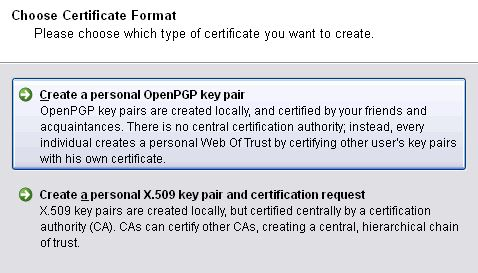
\includegraphics[width=0.8\linewidth]{image/0}}
\caption{Выбор формата сертификата}\label{ris:image0}
\end{figure} 
После чего необходимо заполнить информацию о владельце ключа: имя владельца, адрес электронной почты пользователя, комментарии (опционально). Результат: (Рис. \ref{ris:image1} ).
\begin{figure}[ht]	\center{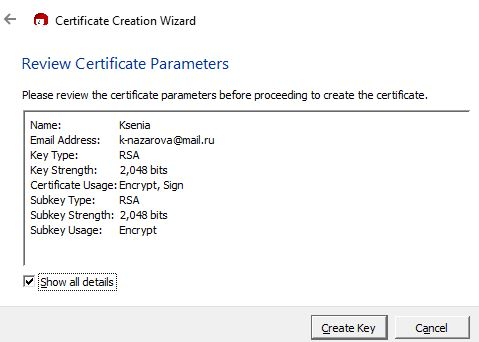
\includegraphics[width=0.8\linewidth]{image/1}}
\caption{Окно для ввода персональных данных.}\label{ris:image1}
\end{figure}
Теперь предлагается ввести фразу-пароль для шифрования закрытого ключа, чтобы он не хранился в явном виде.

Сертификат успешно создан (Рис. \ref{ris:image2} -  \ref{ris:image4}).
\begin{figure}[h]
\center{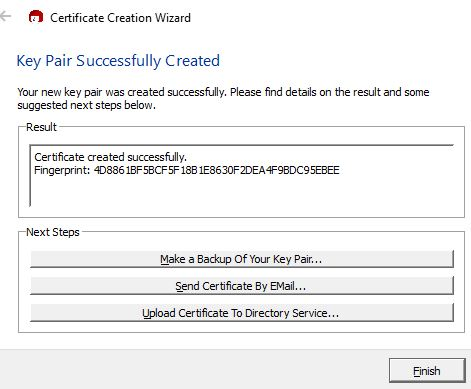
\includegraphics[width=1\linewidth]{image/2}}
\caption{Созданный сертификат}
\label{ris:image2}
\end{figure}
\begin{figure}[h]
\center{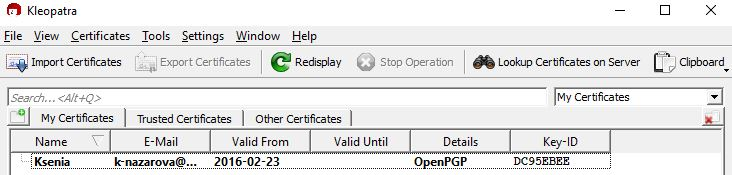
\includegraphics[width=1\linewidth]{image/3}}
\caption{Главное окно \textbf{"Kleopatra"}}
\label{ris:image3}
\end{figure}
\begin{figure}[h]
\center{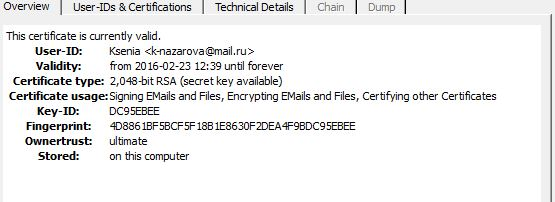
\includegraphics[width=1\linewidth]{image/4}}
\caption{Параметры сертификата}
\label{ris:image4}
\end{figure}


\subsection{Экспорт сертификата}
Для обмена открытыми ключами требуется достать их из программы. Для этого выполняется экспорт сертификата.
Выполним команду \textit{"File ->  Export Certificate"}, в результате чего получим файл с расширением .asc. Это текстовый файл, содержащий созданный ранее открытй ключ:\\

\begin{verbatim}
-----BEGIN PGP PUBLIC KEY BLOCK-----
Version: GnuPG v2

mQENBFbMKNQBCACkB6vR9akfIT25TLnpufqJIF2PiHZNh7uIo8Kd7Waz2JaudKS6
HZ3esLvWALfFpaRye0NTJKeovM80XHcIjvO4LMvcGD21YjA24e0N2o5IM55F2ab1
MN/1k+HS5RSKiXx5ZQat7iZOIvVvatg8Qkd9jBaBrUaIkd1rtkhNkyfY13HPDDEe
QenQJ21Af9gKDN1bQzJC0zYJ6ZKSMbkpBt+tHufkUWi9j//SUE8Hbf6SRLvsq7Ja
TBgwdMDzSG/DvWfzWB/3WwFmf/73J4hIr5crm1eDORIBsqQ/pYfcgjPQE1k9d2Lk
uB5Ae7yEwOwtp6d+DEsWNvDgJpyrT6Z7Z+nXABEBAAG0G0tzZW5pYSA8ay1uYXph
cm92YUBtYWlsLnJ1PokBOQQTAQgAIwUCVswo1AIbAwcLCQgHAwIBBhUIAgkKCwQW
AgMBAh4BAheAAAoJEC3qT5vclevujW0H/RVjpStyNCd73/WfwfGEEaZJZlY1mutc
N1vNR0gUlgkbLnoRFNeeXkkb9tqNuHjhgoOlErpld1OWrqox7VYqADHCOBAzAVsg
A2bRsPkGaGIp1aUQIin8Ubtw+k6A40P03sLhg3g6x/6P23qUJHnmJZrZKoc9ce/z
2+1NZY7ZHOuhYknYC+LH7MdHVvHw/CeKNIwaLvmdTjJJL0U5Gf+aYiziFirMRYb/
MdX430BZRVpelm14Obg/zpXYOs3It1jZh/ZWfPt1u98yY39owfltrKHQFkQw5g2P
iE1lfCdcgW6/Y0tcAEQTGmir1X017nzZZQ1qbhEXFVzpUtbhvWHANfu5AQ0EVswo
1AEIAMLbL9AlNJuo5zw10EyUlZe9B0W6Ls1jG/EaSVCiowv5+GIyqCBUS/Diy3Ot
mSWF8aG37WQPt1OjtcNNasXqJIb9vvZ72qbfiempyYOVWw6jEXpQAgufnaYNK3f+
eWG/OWrdvV4fUBsH9lnQX34LdKtKpY9HpKOryM1h2uQed+EF11ncaGGsKr6bzRf1
A7uLOObou6Ha5VVoeoS7v1VCs3ZHLYTnn4nU7jpUp9e/MTSLHHX8b0P9lhGjc6Ml
6eIfp0RXHEETohEC8eoB/EzOv9FOlLBrobgjlgdkW3T9fPJhGnD/yKk/rXoP5cDL
VE54QoGA7EerbBfCshCVr+4ZFssAEQEAAYkBHwQYAQgACQUCVswo1AIbDAAKCRAt
6k+b3JXr7ri5CACa9KYx7CriSVMgR3UxvWrihu9J8iOYuZcXo51VhYpxEQcee9S0
Qq4HpZRhECkarvmZNROpLP3wKLLONp97tiG0y9eMp03Qz7h20xsRoeJb0h0ZSIdW
N7hNkiJAdsb3ZM8LpCpDQsherO+y1XdckjtSLC7mTI7aaMphL0FDyIqQpQIEIzYd
2mC+tGCA07jEh3lnAKfWlNhlRmDyaG8AJcQyxtWNHVIPKNfHVMnuL8J8i8WBXuhA
53t2v88JVjAwVu8EjoDDv0YfKaCOaoKQDl2RToPvhXhKIjLJC/WXClrxfaMcFnJ5
d+aIC9OwjWAzLg5yPiYUFbihkRcY8dH1Mz5E
=Wyo4
-----END PGP PUBLIC KEY BLOCK-----
\end{verbatim}
Теперь файл можно передать другому пользователю.


\subsection{Поставить ЭЦП на файл}
Для того, чтобы поставить ЭЦП на файл, требуется выполнить следующие действия:
\begin{itemize}
\item Выбрать пункт меню \textit{"File -> Sign/Encrypt Files"}
\item Выбрать файл для шифрования
\item В появившемся окне выбрать действия, которые требуется выполнить
\begin{figure}[h]
\center{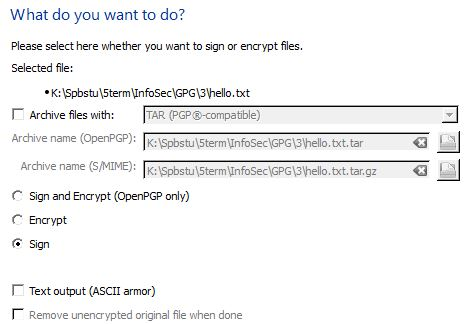
\includegraphics[width=0.6\linewidth]{image/5}}
\caption {Установка ЭЦП на файл}
\label{ris:image5}
\end{figure}
Если установить галку Text output (ASCII armor), то в результате шифрования будет создан не бинарный файл, а текстовый, содержимое из которого можно вставить, например, в текст письма. Если установить галку Remove unencrypted original file when done, то после шифрования исходный файл будет удален.\\
Только для назначения ЭЦП нужно выбрать пункт Sign.
\item Теперь надо выбрать стандарт OpenPGP и сертификат
\begin{figure}[h]	\center{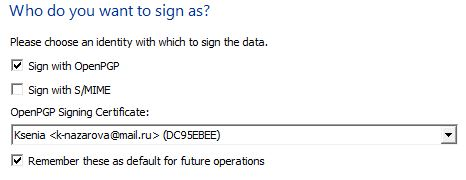
\includegraphics[width=0.8\linewidth]{image/6}}
\caption{Выбор стандарта и сертификата для ЭЦП}
\label{ris:image6}
\end{figure}
\item Ввести фразу-пароль
\begin{figure}[h]	\center{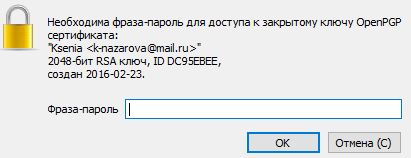
\includegraphics[width=0.8\linewidth]{image/7}}
\caption{Ввод фразы-пароля}
\label{ris:image7}
\end{figure}
\item Установка ЭЦП на файл завершена
\begin{figure}[h]	\center{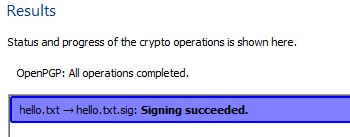
\includegraphics[width=0.8\linewidth]{image/8}}
\caption{Завершение установки ЭЦП}
\label{ris:image8}
\end{figure}
\end{itemize}

\subsection{Обмен зашифрованными сообщениями}
Для начала необходимо импортировать сертификат того, кому планируется отправить сообщение Для этого выполним команду \textit{File -> Import Certificates} и выберем файл, поллученный от коллеги файл с открытым ключом.\\
Теперь выберем файл, зашифруем и подпишем его ЭЦП.\\
\begin{figure}[h]	\center{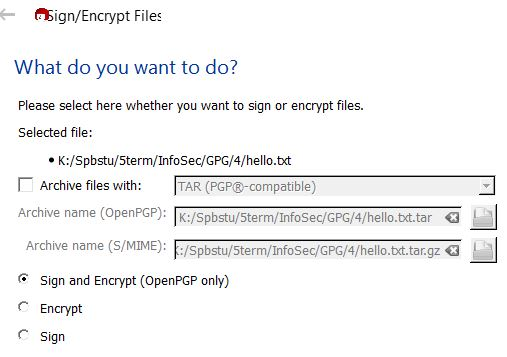
\includegraphics[width=0.8\linewidth]{image/9}}
\caption{Шифрование и установка ЭЦП}
\label{ris:image9}
\end{figure}
Выберем для шифрации полученный открытый ключ владельца, для которого шифруем файл.
\begin{figure}[h]	\center{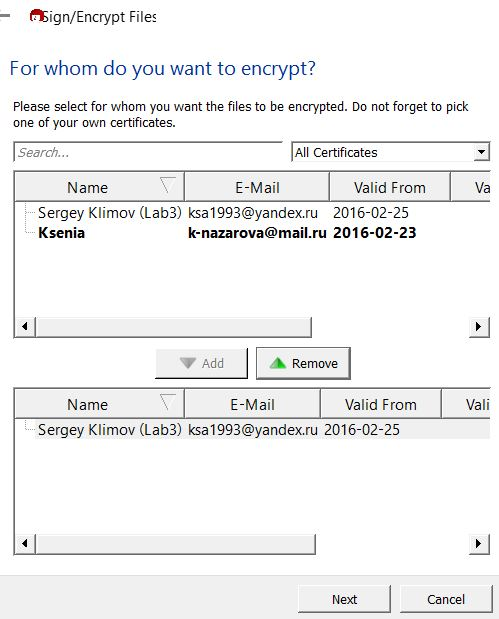
\includegraphics[width=0.7\linewidth]{image/10}}
\caption{Выбор сертификата для шифрования}
\label{ris:image10}
\end{figure}
Теперь выбираем идентификатор, которым устанавливаем ЭЦП на файл.
\begin{figure}[h]	\center{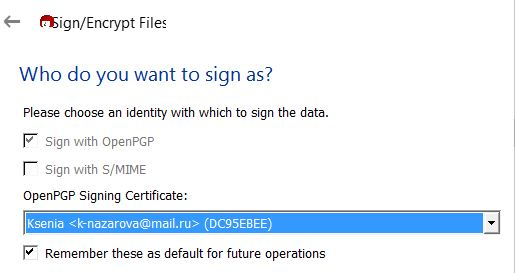
\includegraphics[width=0.7\linewidth]{image/11}}
\caption{Выбор идентификатора для ЭЦП}
\label{ris:image11}
\end{figure}

Теперь файл зашифрован и подписан ЭЦП.
\begin{figure}[h]	\center{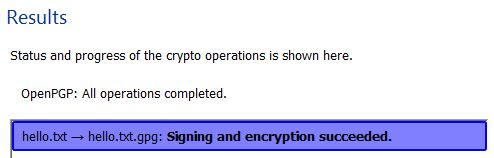
\includegraphics[width=0.7\linewidth]{image/12}}
\caption{Результат}
\label{ris:image12}
\end{figure}

Отправляем зашифрованный файл и срасширением .gpg.
\begin{figure}[h]	\center{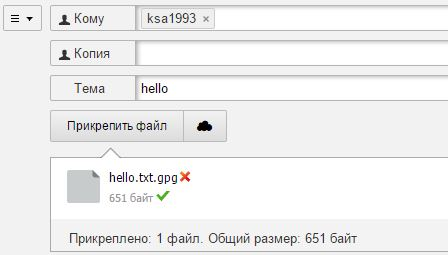
\includegraphics[width=0.7\linewidth]{image/13}}
\caption{Отправка}
\label{ris:image13}
\end{figure}


Получим файл от коллеги,  зашифрованный с помощью нашего открытого ключа. Чтобы расшифровать его, используем наш секретный ключ. Для этого выбираем пункт меню \textit{File -> Decrypt/Verify Files}.
\begin{figure}[h]	\center{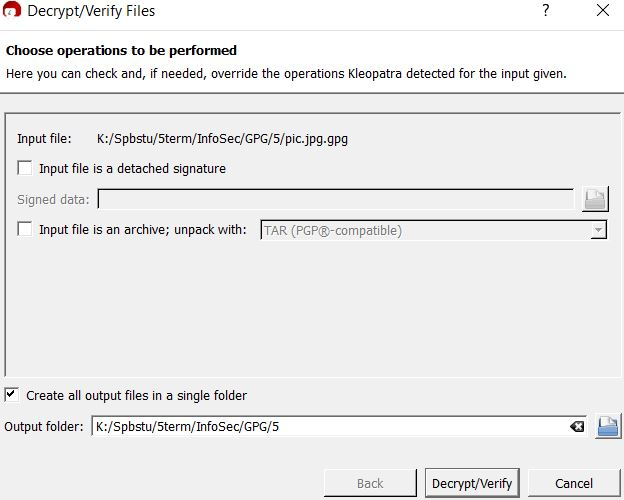
\includegraphics[width=0.7\linewidth]{image/14}}
\caption{Расшифровка чужого файла}
\label{ris:image14}
\end{figure}

\subsection{Использование GNU Privacy handbook}
С помощью GNU Privacy handbook проделаем некоторые действия по использованию gpg через командную строку. \\
Для создания ключевой пары введем в консоле команду \textit{gpg2 --gen-key}. Далее выберем тип ключа, его размер, срок действия, укажем ID пользователя, электронную почту, введем пароль, после чего создастся ключевая пара.  \\
Создали ключ типа RSA и DSA, размером 2048, срок действия которого не ограничен. \\
\begin{verbatim}
C:\Program Files (x86)\GNU\GnuPG>gpg2.exe --gen-key
gpg (GnuPG) 2.0.29; Copyright (C) 2015 Free Software Foundation, Inc.
This is free software: you are free to change and redistribute it.
There is NO WARRANTY, to the extent permitted by law.

Выберите тип ключа:
   (1) RSA и RSA (по умолчанию)
   (2) DSA и Elgamal
   (3) DSA (только для подписи)
   (4) RSA (только для подписи)
Ваш выбор? 1
длина ключей RSA может быть от 1024 до 4096 бит.
Какой размер ключа Вам необходим? (2048)
Запрошенный размер ключа - 2048 бит
Выберите срок действия ключа.
         0 = без ограничения срока действия
      <n>  = срок действия ключа - n дней
      <n>w = срок действия ключа - n недель
      <n>m = срок действия ключа - n месяцев
      <n>y = срок действия ключа - n лет
Срок действия ключа? (0)
Срок действия ключа не ограничен
Все верно? (y/N) y

GnuPG необходимо составить ID пользователя в качестве идентификатора ключа.

Ваше настоящее имя: Ksenia
Адрес электронной почты: k-nazarova@mail.ru
Комментарий:
Вы выбрали следующий ID пользователя:
    "Ksenia <k-nazarova@mail.ru>"

Сменить (N)Имя, (C)Комментарий, (E)Адрес или (O)Принять/(Q)Выход? o
Для защиты закрытого ключа необходима фраза-пароль.

Необходимо получить много случайных чисел. Желательно, чтобы Вы
в процессе генерации выполняли какие-то другие действия (печать
на клавиатуре, движения мыши, обращения к дискам); это даст генератору
случайных чисел больше возможностей получить достаточное количество энтропии.
Необходимо получить много случайных чисел. Желательно, чтобы Вы
в процессе генерации выполняли какие-то другие действия (печать
на клавиатуре, движения мыши, обращения к дискам); это даст генератору
случайных чисел больше возможностей получить достаточное количество энтропии.
gpg: ключ D88F431B помечен как абсолютно доверенный.
открытый и закрытый ключи созданы и подписаны.

gpg: проверка таблицы доверия
gpg: требуется 3 с ограниченным доверием, 1 с полным, модель доверия PGP
gpg: глубина: 0  верных:   2  подписанных:   0  доверие: 0-, 0q, 0n, 0m, 0f, 2u
pub   2048R/D88F431B 2016-03-20
      Отпечаток ключа = 223A FA09 83B4 78D2 B7CB  49E4 FBD9 0CC6 D88F 431B
uid     [абсолютное] Ksenia <k-nazarova@mail.ru>
sub   2048R/716EFD07 2016-03-20
\end{verbatim}
 
Чтобы посмотреть список всех имеющихся сертификатов, используем команду  \textit{gpg --list-key}. Видим в списке все ключи, созданные или импортированные как в графической оболочке, так и в консоле (рисунок \ref{ris:image18} ).
\begin{verbatim}
C:\Program Files (x86)\GNU\GnuPG>gpg2.exe --list-key
C:/Users/Kseniya/AppData/Roaming/gnupg/pubring.gpg
--------------------------------------------------
pub   2048R/DC95EBEE 2016-02-23
uid     [абсолютное] Ksenia <k-nazarova@mail.ru>
sub   2048R/AD121C7E 2016-02-23

pub   2048R/C75B147B 2016-02-25
uid     [неизвестно] Sergey Klimov (Lab3) <ksa1993@yandex.ru>
sub   2048R/409CA923 2016-02-25

pub   2048R/D88F431B 2016-03-20
uid     [абсолютное] Ksenia <k-nazarova@mail.ru>
sub   2048R/716EFD07 2016-03-20

pub   2048R/C4C7C913 2016-03-20
uid     [абсолютное] Ksenia3 <knazarova9@yandex.ru>
sub   2048R/AD6D09B7 2016-03-20 
\end{verbatim}

Для шифрации и подписи ЭЦП документа для какого-либо другого пользователя (в данном случае, для Sergey Klimov (Lab3)) используем команду \textit{gpg2 -se -r "Sergey Klimov (Lab3)" }.
\begin{verbatim} 
C:\Program Files (x86)\GNU\GnuPG>gpg2.exe -se -r "Sergey Klimov (Lab3)" K:\Spbstu\5term\InfoSec\GPG\
im.jpeg

Необходима фраза-пароль для доступа к закрытому ключу пользователя: "Ksenia <k-nazarova@mail.ru>"
2048-битный ключ RSA, ID DC95EBEE, создан 2016-02-23

gpg: 409CA923: Нет свидетельств того, что данный ключ принадлежит названному пользователю

pub  2048R/409CA923 2016-02-25 Sergey Klimov (Lab3) <ksa1993@yandex.ru>
 Отпечаток главного ключа: C1B5 3092 2541 E7C1 F4C9  56A0 FCE8 1058 C75B 147B
       Отпечаток подключа: 8949 D6B8 413D F7AF 6C18  0625 E03B 046B 409C A923

Нет уверенности в том, что ключ принадлежит человеку, указанному
в ID пользователя ключа. Если Вы ТОЧНО знаете, что делаете,
можете ответить на следующий вопрос утвердительно.

Все равно использовать данный ключ? (y/N) y
\end{verbatim}
В результате создается зашифрованная копия документа с расширением .gpg.

Экспорт своего открытого ключа выполняется при помощи команды \textit{gpg2.exe --armor --export knazarova9@yandex.ru}
\begin{verbatim}
C:\Program Files (x86)\GNU\GnuPG>gpg2.exe --armor --export knazarova9@yandex.ru
-----BEGIN PGP PUBLIC KEY BLOCK-----
Version: GnuPG v2

mQENBFbu+F8BCACds4Yt2c9iUVX5VdoeuHv+5X4By7xPoJ1sawu6LiDatuEhZKG/
4th0deNzLD9nX/Myd/XoAPoun/2Fy/HVLvuBkh8ZaNnO3+p7FoTo9DZRGpFLgICp
oCgY8cdU1SnwLGcUBHcmcHnC2ExCVLxRGV1iCCCCpuL5E5WNURll1yLJPsYlF3r9
+uVt4f/dn8xZFJQrBwz3MRywleCbz8HnEFcUFme52Qig9gLZ6v0d3uvT6iXZWwlB
ESkQbuyIYfa56/vNvOuKDj+kgGix46/mScdPqcdVWFT3hpdthnMzv9Hf0yADdW0F
uPfZuqJ+yxILiL0uX45MtyTqoOy+xN4cwKuFABEBAAG0HktzZW5pYTMgPGtuYXph
cm92YTlAeWFuZGV4LnJ1PokBOQQTAQgAIwUCVu74XwIbAwcLCQgHAwIBBhUIAgkK
CwQWAgMBAh4BAheAAAoJENeK5WnEx8kT0v0H/icz3VhqFoBB1z63Hu4T5GLs/wxE
P8s9HLGXHJxfTTbkBQMKXTGisw1wOTiWwIuA6NcFCBujCuJ6lZgEFdKfqiQiof/s
Y3b0TkriZ9hAL0tP7dpzbVB8v0jf6Sl5eoLPnhENVZnCXE7GGEYk6uDByZIK0OJg
tj1svfuUyAryanXazAKowv4AzDq8MJmQCMD5qP3cI3rmohJRrodO7Y8TwE59cz5Y
LCasjtCKheuKYKlr3ZDmwNyv8HIkKzLMbqZ7hZSQc4rsOfjqCa6tJpDpApWvA5To
DkVren3zIz6NC6iST2jqsJSXTenRE0Vv1Ci3RUeOcQwi67TipY4Hj3BOJau5AQ0E
Vu74XwEIAOI4EeHVGKS8zVbAp8Wkkj88mlvniJWc+Afecumwvk4JFozX/CfkGSuk
VgIiMaHxnALjHvBFckKukl6vM20gslvEa3R3LvKZ+5oVkPtAIBbsoFKADqG9Pp6p
bL0YvxC/scKNv9PbB6j0G6o8Q3eh1wvnsP7Qr2sSS/OK+o3S7v0tCaJyufUtOVuQ
gWcC//pdox2R+s1xVS2AFeX+Q7P76EnXtkPKC+saADmOC+fkH2vQtW+iOhLHIMH+
aVQLxKTiEfr/qK1M/YKZjzs8EGKd6zEhAzg4kz8hZF/IaNOiihm59DwzYZvPbQPh
myxa8q7Uxq49WMlg4dCMdPlm8R8Uxo8AEQEAAYkBHwQYAQgACQUCVu74XwIbDAAK
CRDXiuVpxMfJE3IUCACSGEkpCThArxdJMiqZptjElSy11g6EM8qSHpKWcL4xmOa9
f6f7d5jrOoaDmQwuWNmrFi/9qxj0NGhgu24YegQe5Cm/Vv+pG7E+9qS7kal7PayV
kfpVtUQ8nNVsJVWaQJeYN7i5u1hbEAjvtDq3VlaMlXhFiEauCA1SyuiyT/cRxG/D
+zy8totrHOdEyF1zk4w6zzQNqczz7ZRlQtdn4gvyg/ESbiqgT9w/Q2cP5PY/Zauo
4/2+hYuIOGMT6alzutWAh9jGRJc/JxMBKbuxXuWEX2EPgUo4+HbQxDwjXhM8XlXn
NsDoilrJwH0e3IWTbMkWxVQStB/qEKN1hLWG2jqM
=5EHM
-----END PGP PUBLIC KEY BLOCK-----
\end{verbatim}
\section{Вывод}
В ходе лабораторной работы, используя пакет Gpg4win, я научилась создавать собственные ключевые пары и сертификаты на них; подписывать файлы и проверять подпись, а также зашифровывать и расшифровывать документы с помощью собственного сертификата или стороннего. Вышеперечисленные действия легко произвести как из графической обочки \textbf{Kleopatra}, так и из командной строки. 
\end{document}